\section{Durchführung}
\label{sec:Durchführung}

Bevor der Doppler-Effekt bestimmt werden kann, müssen zunächst die Grundfrequenz des Lautsprechers, die Geschwindigkeit des Wagens in seinen verschiedenen Gängen,
und die Schallgeschwindigkeit im Versuchsraum bestimmt werden. Ersteres kann zwischen den Wertenahmen im letzten Versuchsteil geschehen.


\subsection{Bestimmung der Wagengeschwindigkeit}
\label{sub:Bestimmung der Wagengeschwindigkeit}
Zur Vorbereitung der ersten Messung soll zunächst eine geeignete Schaltung entworfen werden, die mihilfe des Mikorsekunden-Zählers eine Stopuhfunktion erzeugt,
und deren Start und Stop an die Lichtschranken küpft. Zunächst sollen die einzelnen Geschwindigkeiten des Wagens in verschiedenen Gängen gemessen werden.
Dafür werden die Lichtschranken in genügendem Abstand zueinander platziert und eine von ihnen als Auslöser die andere als Stoppsignal an die Schaltung geschlossen werden
(Die Messung der Rücklaufgeschwindigkeit muss danach mit gewechselten Rollen durchgeführt werden).
Zur schlussendlichen Bestimmung der Geschwindigkeit des Wagens muss auch noch die Strecke zwischen den beiden Lichtschranken mit einem Maßband gemessen werden.
\begin{figure}
  \centering
  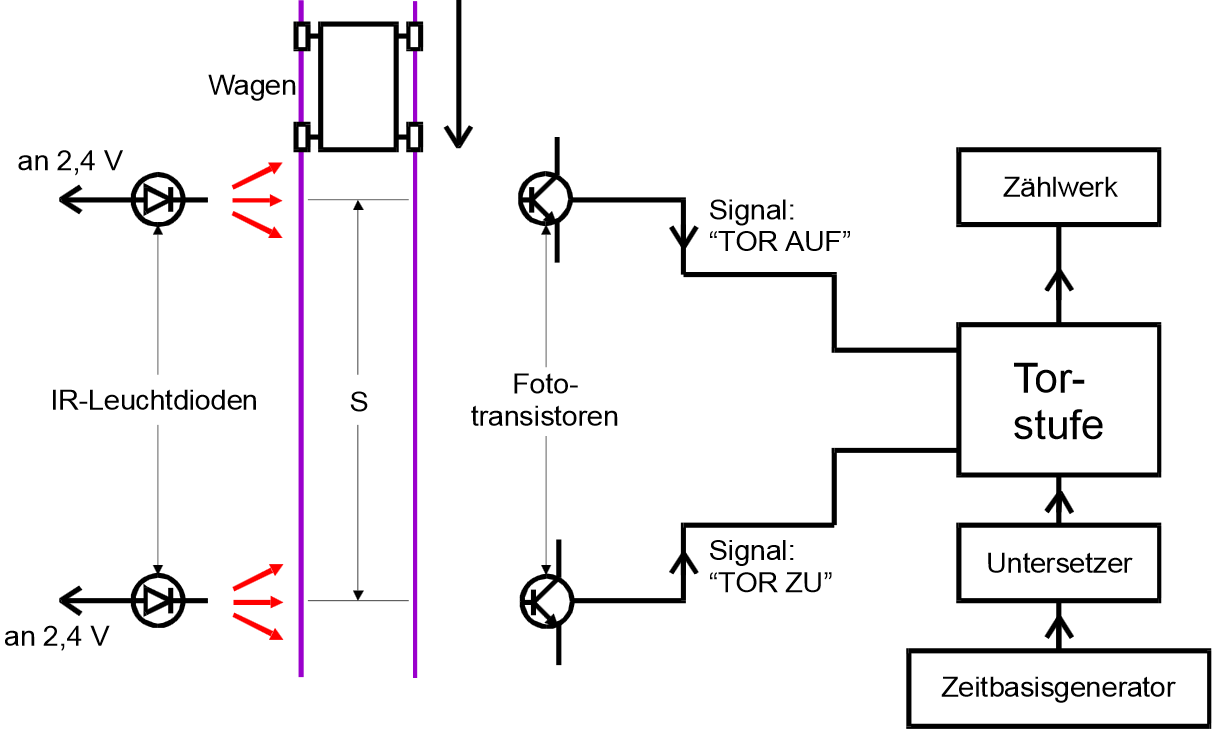
\includegraphics[width=\textwidth]{Geschwindigkeit.png}
  \caption{Versuchsaufbau zur Geschwindigkeitsmessung}
  \label{fig:Geschw}
\end{figure}
In der notwendigen Schaltung muss zuanfang der Zeitbasisgenereator, der hochpräzise
Impulse im $ \num{1} \si{\micro\second} $  Takt erzeugt, mit dem Untersetzer verbunden werden,
der diese in regelbar verschiedenen Zehnerpotenzen zusammenfasst. In der Torstufe
werden beide Signale der Lichtschranken mit einem Schmitt-Trigger verneint,
dann über einen Flip-Flop zusammengeführt und mit dem zuvor erwähnten UND-Gatter verbunden.
Es ist außerdem noch eine sinnvolle Übersetzung des Unterstetzers zu wählen.Dieser wird dann zusammen mit dem was mit "Torstufe" betitelt ist (\ref{fig:Geschw}) an ein UND-Gatter angeschlossen.
In dieser Tor Stufe werden beide Signale der Lichtschranken mit einem Schmitt-Trigger verneint, dann über einen Flip-Flop zusammengeführt und mit dem zuvor erwähnten UND-Gatter verbunden.
Es ist außerdem noch eine sinnvolle Übersetzung des Unterstetzers zu wählen.


\subsubsection{Bestimmung der Schallgeschwindigkeit}
\label{subs:Bestimmung der Schallgeschwindigkeit}
Für die präzise Messung der Schallgeschwindigkeit wird nun ein auf eine Schiene montierter Präzisionsschlitten genutzt, auf dem der Lautsprecher befestigt wird.
Ein Oszilloskop wird mit einem Ausgang mit dem Frequenzerzeuger und mit dem anderen mit dem Mikrophon verbunden, was dem Lautsprecher gegenüber auf der Schiene angebracht wird.
Nun wird die Zweikanaleinstellung des Oszilloskopes genutzt um die Lissajous-Figur zu erzeugen. Das Ziel ist es nun diese Figur auf eine einzige Linie umzuformen.
Ist dies gelungen so verschiebt man den Lautsprecher weiter, sodass eine Linie in die andere Richtung zu sehen ist. Der Abstand um den der Lautsprecher verschoben wurde ist dann die halbe Wellenlänge.

\begin{figure}
  \centering
  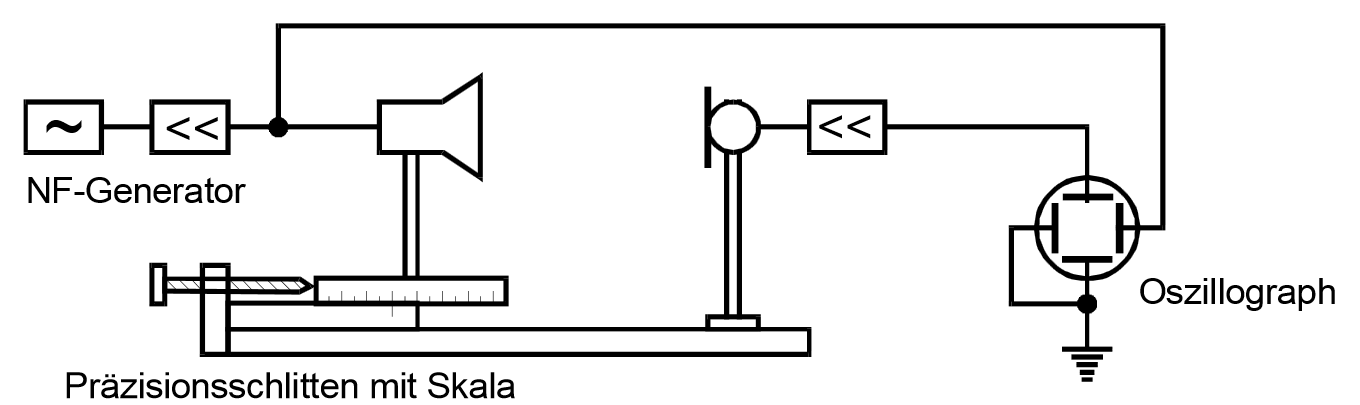
\includegraphics[width=\textwidth]{Schallgeschwindigkeit.png}
  \caption{Versuchsaufbau zur Schallgeschwindigkeitsmessung}
  \label{fig:Schall}
\end{figure}

\subsubsection{Doppler-Effekt}
\label{subs:Doppler-Effekt}
Zur Messung zum Doppler-Effekt muss nun die Schaltung aus der ersten Messung modifiziert werden, sodass nun(

)
So geschaltet wird jetzt also immer genau eine Sekunde lang gemessen (sofern die richtige skalierung gewählt ist),
nachdem die vordere Lichtschranke durchbrochen wurde und gemessen werden die Impulse die aus dem Mirkophon empfangen werden.
Die angezeige Zahl ist also genau die Frequenz in $\si{\Hertz}$. Für die eigentliche Messung muss nun der Lautsprecher auf den Wagen geschraubt werden und das Mikrophon in description
Halterung am dente der Wagestrecke angebracht werden, sodass sich der Wagen darauf zu und davon weg bewegt.


\begin{figure}
  \centering
  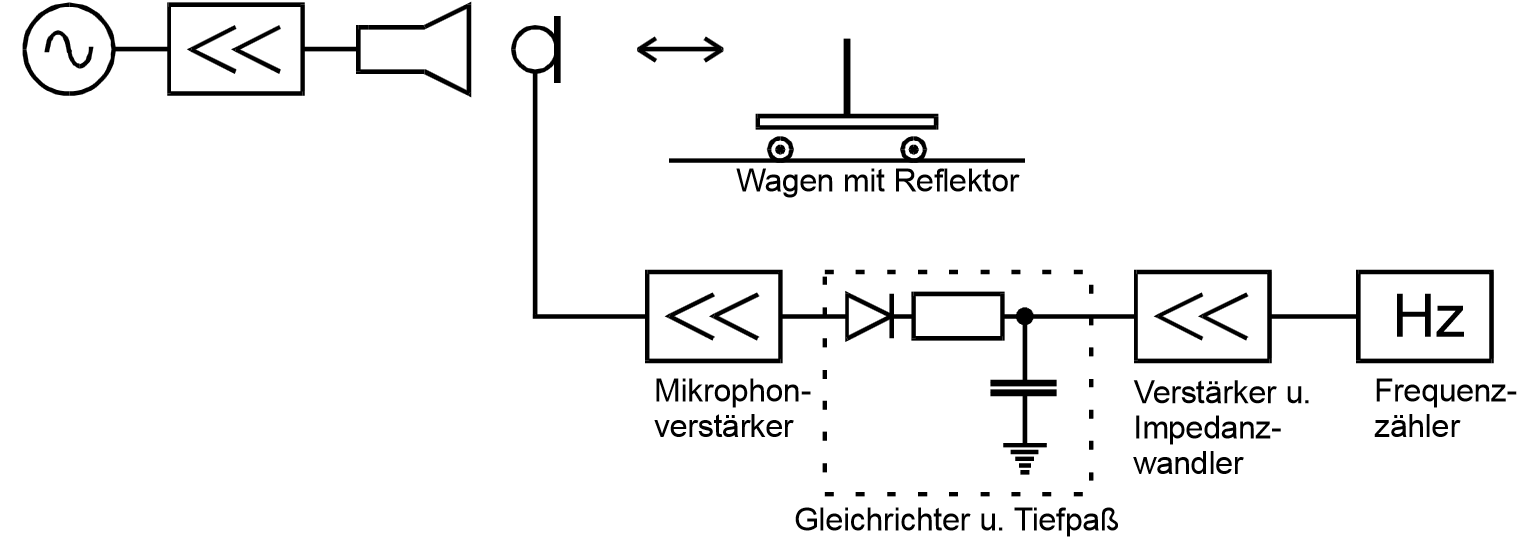
\includegraphics[width=\textwidth]{Wand.png}
  \caption{Versuchsaufbau zur Messung Doppler-Effekt durch Schwebungen}
  \label{fig:Schall}
\end{figure}


In der letzten Messung muss die Schaltung nun an anderer Stelle verändert werden, dass nun zwischen dem Mikrophon und dem Zähler ein Gleichrichter und Tiefpass,
sowie ein Impedanzwandler zwischengeschaltet werden muss, der für uns die Frequenzdifferenzen isoliert damit wir diese anzeigen lassen können.
Anstelle des Lautsprechers, der jetzt neben dem Mikrophon befestigt ist, ist jetzt eine Metallplatte auf dem Wagen angebracht die den Schall von dem Lautsprecher aus reflektiert.
Damit er ins Mikrophon fällt muss man einige Feinjustierung vornehmen, da der Mikorphonkopf sehr klein ist, es aber bei sich leicht änderndem Reflexionswinkel die ganze Zeit empfangen soll.
